\chapter{Operando EPR Spectroscopy of TEMPO-Salen Cathode Films}
\section{Electron Paramagnetic Resonance}
\subsection{The Spin Hamiltonian}
\paragraph*{Electron Spin}
The electron bears an internal angular momentum that is called spin. Spin combines with the charge of the electron to endow the electron with a magnetic moment. The magnetic moment of the electron is quantized: $\mu_e=\mu_BgS$ \cite{SternGerlach1922}, where $S$ is the spin quantum number, the eigenvalue of the spin operator $\vec{\hat{S}}$, that equals $S=1/2$ for an electron. When an electron is placed in a static magnetic field $\vec{B_0}=B_0 \vec{e_z}$, its magnetic moment precesses about the field direction with the Larmor frequency $\omega_L = \gamma B_0$, where $\gamma=\frac{g_e\mu_B}{\hbar}=28.025$~GHz/T is the gyromagnetic ratio of the electron and $g_e$ is the electron g factor. The projection of the electron's magnetic moment on the direction of the magnetic field can take only discrete values between $-S=-1/2$ and $S=1/2$, so that the eigenvalues of the $z$ component of the spin operator are also discrete: $\hat{S}_Z\vert{\uparrow\rangle}=+\frac{\hbar}{2}\vert{\uparrow\rangle}$, $\hat{S}_Z\vert{\downarrow\rangle}=-\frac{\hbar}{2}\vert{\downarrow\rangle}$. The two eigenfunctions of $\hat{S}_Z$ are called the spin-up state $\vert{\uparrow\rangle}$ and the spin-down state $\vert{\downarrow\rangle}$. The two corresponding eigenvalues $\pm\frac{\hbar}{2}$ define the energy difference between the states $\vert{\uparrow\rangle}$ and $\vert{\downarrow\rangle}$, that is known as the Zeeman splitting.

\paragraph*{Zeeman Splitting}
The energy of an unpaired electron placed in the external magnetic field $\vec{B_0}$ is the eigenvalue of the spin Zeeman Hamiltonian: $\hat{H}_{EZ} = \mu_B g\vec{B}_0\cdot\vec{\hat{S}}$. In the laboratory frame of reference $\vec{B_0}\parallel\vec{e_z}$, $\left[\hat{H}_{EZ},\hat{S}_z\right]=0$, so $\hat{H}$ and $\hat{S}_Z$ share the eigenfunctions $\vert{\uparrow\rangle}$ and $\vert{\downarrow\rangle}$. The Zeeman energies of the electron are $E_{EZ}^{\pm} = \pm \frac{\hbar}{2}\mu_B g B_0$. 

\paragraph*{Nuclear Spin and Nuclear Zeeman Splitting}
A proton also bears an internal angular momentum $S=1/2$ that results in a magnetic moment $\mu_p = \mu_e\frac{m_e}{m_p}$, that is $\frac{m_e}{m_p}\approx1836$ times smaller than the electron's magnetic moment. A neutron bears no charge but still has an internal angular momentum $S=1/2$. An atomic nucleus that consists of protons and neutrons can have a magnetic moment, depending on the mutual orientations of their spins and on the nuclear charge. A nitrogen nucleus has 7 protons and 7 neutrons that total in a nuclear spin $I=1$ which, with the g factor for the nitrogen nucleus $g_N$, results in the nuclear magnetic moment of $\mu_N=\mu_Bg_N\frac{m_e}{m_N}I$ that splits into three Zeeman energy levels corresponding to $I=-1,0,+1$, analogously to the electron with $S=1/2$. The nuclear Zeeman splitting is more than three orders of magnitude weaker than the electron Zeeman splitting because of the difference in the masses of the particles.

\paragraph*{Hyperfine Interaction}
The magnetic moments of an electron and a magnetic nucleus, such as nitrogen, couple in the hyperfine interaction~\cite{Schweiger2001_hfi}: $H_{HF}=\vec{\hat{S}}\textbf{A}\vec{\hat{I}}=H_F+H_{DD}$ with the hyperfine tensor $\textbf{A}$. The isotropic part $H_F=a_{iso}\vec{\hat{S}}\vec{\hat{I}}$, or the Fermi contact interaction, scales with the probability density of the electron at the position of the nucleus $a_{iso}=\frac{2}{3}\frac{\mu_0}{\hbar}g_e\beta_eg_n\beta_n\vert\psi(0)\vert^2$. The anisotropic part $H_{DD}=\vec{\hat{S}}\textbf{T}\vec{\hat{I}}$ with the dipolar coupling tensor $\textbf{T}$ takes into account the anisotropic dipole-dipole coupling between the magnetic moments of the electron and the nucleus.

\paragraph*{Nuclear Quadrupole Moment}
The nitrogen nucleus has a spin greater than 1/2 which alters the charge distribution within the nucleus which gives rise to a non-vanishing nuclear electrical quadrupole moment $Q$. The interaction between the asymmetrically distributed charge and the gradient of the electric field at the nucleus is given by the nuclear quadrupole Hamiltonian $H_{NQ}=\vec{\hat{I}}\textbf{P}\vec{\hat{I}}$ with the nuclear quadrupole tensor $\textbf{P}$ that describes the coupling of the nuclear quadrupole moment to the electric field gradient.

\paragraph*{Exchange Interaction}
In a system of closely placed electrons, such as in a film of densely packed nitroxide radicals, the electron orbitals may overlap significantly and the radicals may exchange electrons. The energy required to exchange the electrons is called the Heisenberg exchange coupling $H_{exch} = \vec{\hat{S_1}}\textbf{J}\vec{\hat{S_2}}$, that becomes considerably large at inter-spin distances below $r<1.5$~nm or with a large spin delocalization~\cite{Schweiger2001_exch}. The positive $\textbf{J}$ corresponds to a weak coupling between $S_1$ and $S_2$ which leads to an antiferromagnetic or antiparallel alignment of spins with a total $S=0$, whereas the negative $\textbf{J}$ causes the strong inter-spin coupling which leads to a ferromagnetic alignment with $S=1$.

\paragraph*{Magnetic Dipole-Dipole Interaction}
The dipole-dipole interaction between the two neighboring electron spins contributes one more term to the spin Hamiltonian: $H_{dd} = \vec{\hat{S_1}}\textbf{D}\vec{\hat{S_2}}$ that depends on the distance between the spins. 

\subsection{Instrumentation}
\paragraph{EPR Hardware}
First observed in 1943, the phenomenon of electron paramagnetic resonance had become a tool for probing local molecular environments in species that contain an unpaired electron that experiences the Zeeman splitting in a constant magnetic field $B_0$. A free electron, that does not interact with its environment and has $g=g_e$, experiences a Zeeman splitting of $\Delta E = g \mu_B B_0$, that corresponds to the energy of a photon with a frequency of $\nu=\Delta E / h$. At $B_0\approx0.3$~T, a microwave photon with $\nu\approx9.5$~GHz can drive the magnetic dipole transition between $\vert{\uparrow\rangle}$ and $\vert{\downarrow\rangle}$, that is called the spin flip. The microwave sources are historically\cite{RADARS} available in a number of discrete bands, one of them is known as $X$ band for the range between 8 and 12 GHz. To ensure that only the magnetic component of the microwave photon is interacting with the sample, a resonating cavity is used, where a standing microwave is formed, so that in the center of the cavity, the magnetic component of the microwave is maximized and the electric component is quenched. The sample is inserted in the center of the cavity and the external magnetic field is sweeped. When the resonance condition is met~\ref{eq:RESONANCE_CONDITION}, the spin flip occurs and the photon is being absorbed by the sample. The resonance absorption of microwaves can be detected by a small decrease in the quality factor $Q$ of the resonating cavity, as the magnetic field is being scanned and the microwave frequency is kept constant. The change in the $Q$ factor during the spin flip leads to temporal decoupling of the resonator, that causes reflections of the microwave that would have entered the resonator off resonance. The intensity of the microwaves is measured with a biased semiconductor diode that has a linearly changing conductivity in the range corresponding to  the incident microwave power. A phase sensitive detection with the shallow modulation of $B_0$ increases the signal-to-noise ratio (SNR), and yields the derivative of the resonance absorption profile. The typically high $Q\gg1$ factor of the resonating cavity further increases the SNR.


\section{EPR Spectroscopy of a Charging Electrochemical Cell}

\subsection{Fabrication of EPR-compatible Electrochemical Cells}

\subsection{EPR Spectra During a Charge-Discharge Cycle}

\subsection{Spectral Simulations}

\subsection{Quantitative Analysis of Potential-Dependent EPR Spectra}

\subsection{EPR-Detected State Of Charge}

\subsection{Formation of Singlet Spin States in a Reduced Cathode Film}

\subsection{Monitoring of Degradation Processes}

\subsection{Monitoring of Self Discharge}

\subsection{Electrochemical Cells with Solid Electrolyte}

\subsection{Low Temperature Measurements}
\begin{figure}[h]
\center
	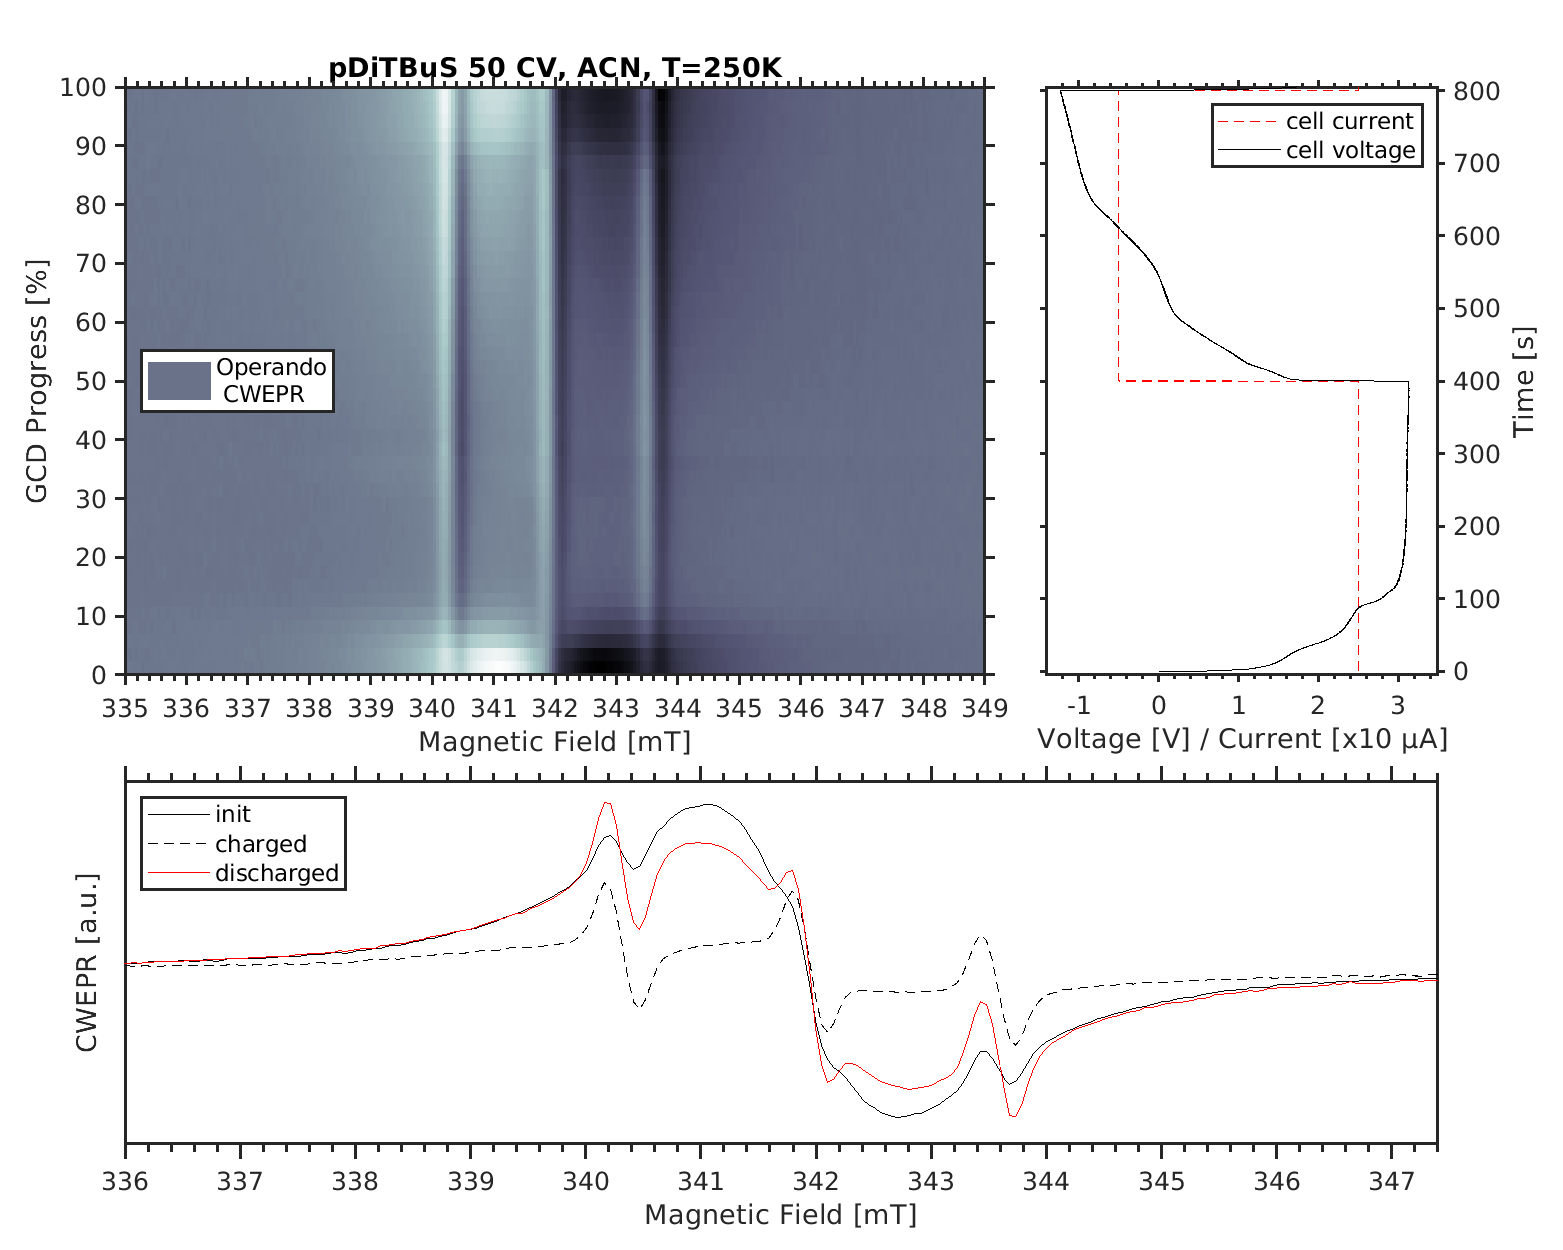
\includegraphics[width=1\textwidth]{./operando_epr/figures/slowcharge_231117_liquid_250K.pdf}
	\caption{XXX}
	\label{fig:Figure_1}
\end{figure}

